This section describes the sound program, and details how it was developed. This section covers procedure, setup and configuration, tools and program details.

need to include a bit about the Makefile here


\section{Functional Description}
	The solution program plays sound effects and music, and is controlled by the eight buttons on the STK1000.
The LEDs are used to indicate which sound is playing.

When the program is started, the board is in idle mode, ready to react to button presses.
Pressing any of the buttons \texttt{SW0}-\texttt{SW3} plays a piece of music, which loops until another sound is selected.
Pressing any of the buttons \texttt{SW4}-\texttt{SW6} plays a sound effect, which is not looped.
Pressing \texttt{SW7} stops all playback.

\subsection{Sound effects}

The sound effects are generatively composed by wrapping a generator signal in a configurable ADSR volume envelope.
Because the internal DAC of the STK1000 is rather noisy because of signal bleeding and poorly implemented hardware filters, the sound from the generators can sound rather dirty.

The available generator signals in the program are NOISE, SAWTOOTH and SQUARE.

A sawtooth wave is a wave that increases linearly, until it cuts off, as seen in figure \ref{img-sw5zoom}.
The sawtooth wave includes all the integer harmonics for the given frequencies.
\begin{figure}[H]
	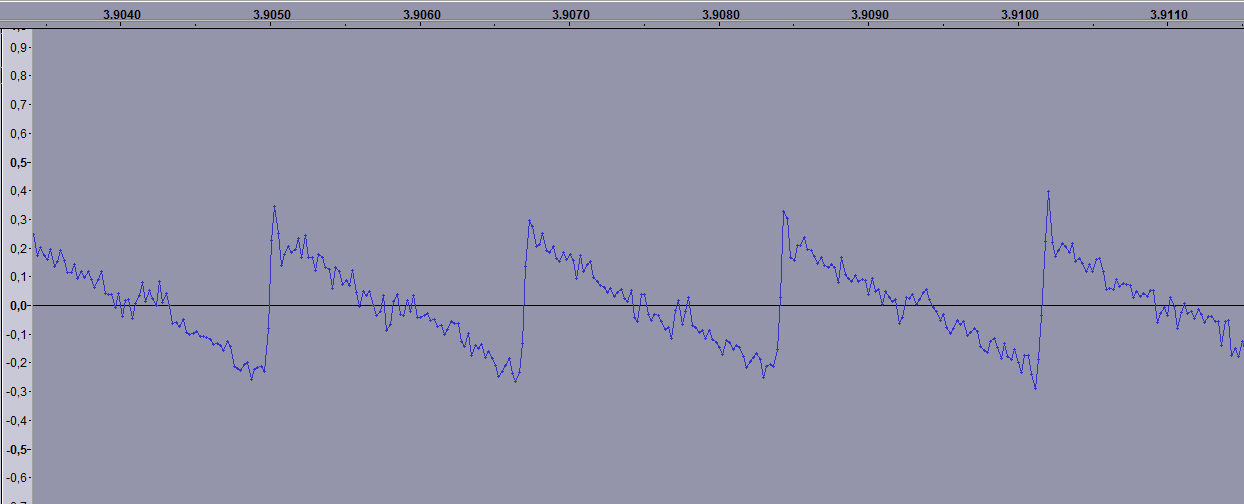
\includegraphics[width = \textwidth]{images/SW5zoom.png}
	\caption{A noisy sawtooth wave recorded from the STK1000.}
	\label{img-sw5zoom}
\end{figure}

An ideal square wave is either at a maximum or minimum amplitude as seen in figure \ref{img-sw4zoom}, and shifts between them instantly.
Unlike a sawtooth wave, the square wave only contains odd-numbered integer harmonics.
\begin{figure}[H]
	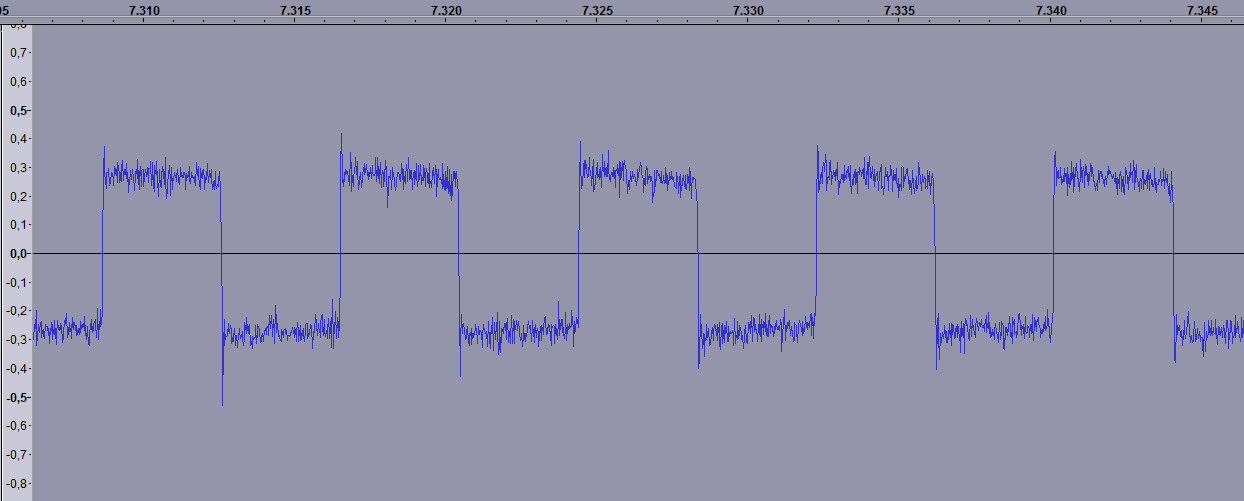
\includegraphics[width = \textwidth]{images/SW4zoom.png}
	\caption{A noisy square wave recorded from the STK1000.}
	\label{img-sw4zoom}
\end{figure}

A noise is rather the lack of a waveform, with randomly chosen samples, as depicted in figure \ref{img-sw6zoom}.
Noise can be described as the sound your tv makes when you tune into frequencies that there is no broadcasting on.
\begin{figure}[H]
	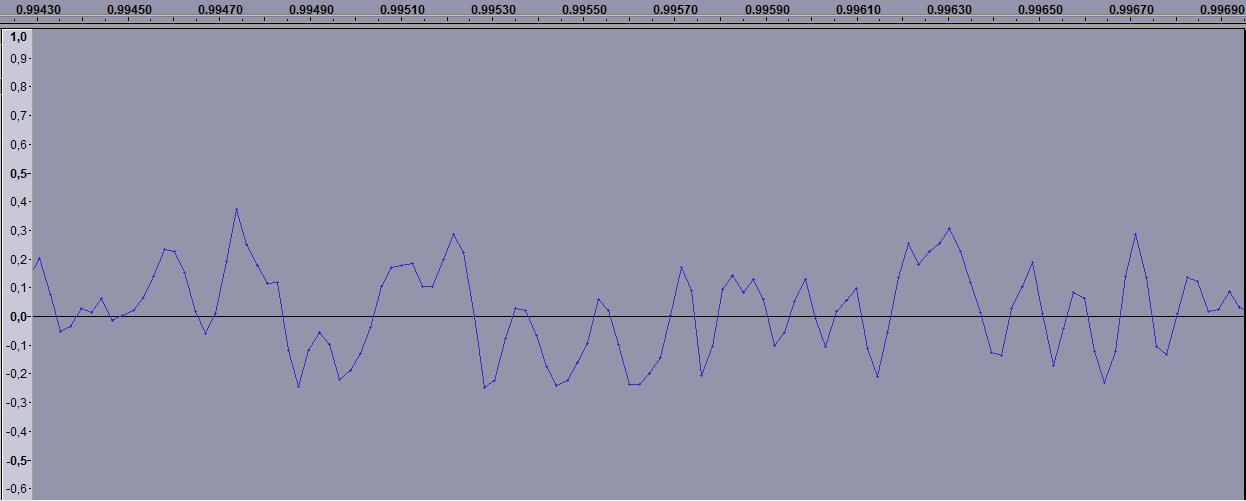
\includegraphics[width = \textwidth]{images/SW6zoom.png}
	\caption{A noise signal recorded from the STK1000}
	\label{img-sw6zoom}
\end{figure}

In order to make sound effects we need more than just pure waves, as sound almost never consists of just a wave with constant amplitude.
It is the job of the ADSR envelope to solve this issue.
An envelope sets bounds for the amplitude of a wave, and an ADSR envelope divides the wave into four parts: attack, decay, sustain and release.

During the attack, the amplitude is gradually increased from 0 to a maximum value.
After the attack, the amplitude gradually decays to a sustain level, which is typically a fraction of the maximum value.
The sound stays at the sustain level for a given time, until it is released, and the amplitude gradually decreases until it reaches 0 again.

\subsubsection{Explosion}

`Explosion' is a NOISE-based sound effect with the following ADSR envelope:
\begin{itemize}
	\item{Attack: 0 ms}
	\item{Decay: 1000 ms}
	\item{Sustain: 0\%}
	\item{Release: 0 ms}
\end{itemize}
The effect is held for 0 ms.
The total length of the effect is $0 ms + 1000 ms + 0 ms + 0 ms = 1000 ms$.
`Explosion' can be triggered by pressing \texttt{SW6}.
The sound effect is depicted in figure \ref{img-sw6}.

\begin{figure}[H]
	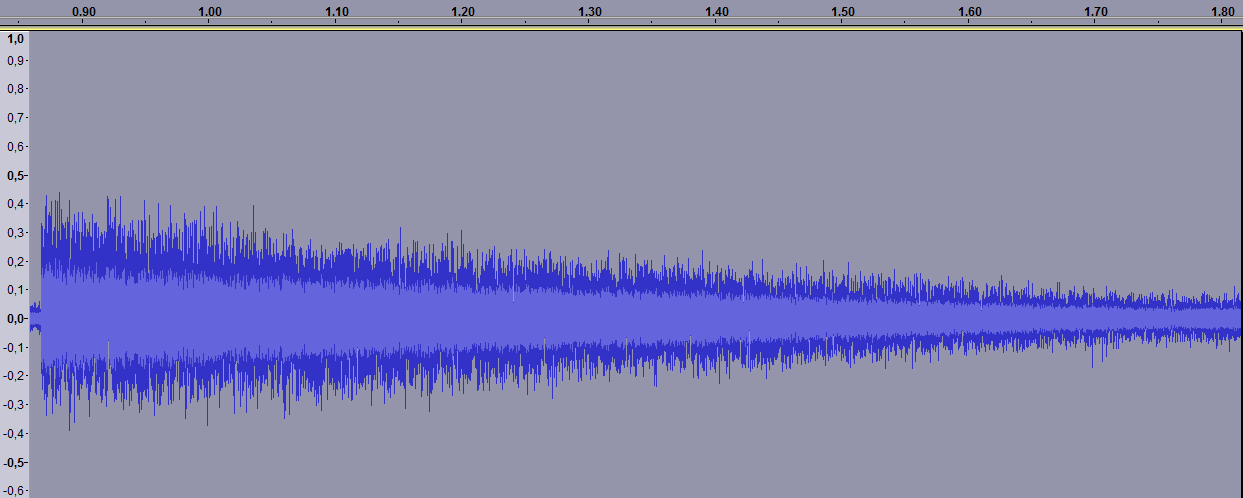
\includegraphics[width = \textwidth]{images/SW6.png}
	\caption{}
	\label{img-sw6}
\end{figure}


\subsubsection{Air horn}
`Air horn' is a SAWTOOTH-based sound effect with the following ADSR envelope:
\begin{itemize}
	\item{Attack: 100 ms}
	\item{Decay: 100 ms}
	\item{Sustain: 70\%}
	\item{Release: 500 ms}
\end{itemize}
The effect is held for 0 ms.
The total length of the effect is $100 ms + 100 ms + 500 ms + 0 ms = 700 ms$.
`Air horn' can be triggered by pressing \texttt{SW5}.
See figure \ref{img-sw5} for a visualization of `Air horn'.

\begin{figure}[H]
	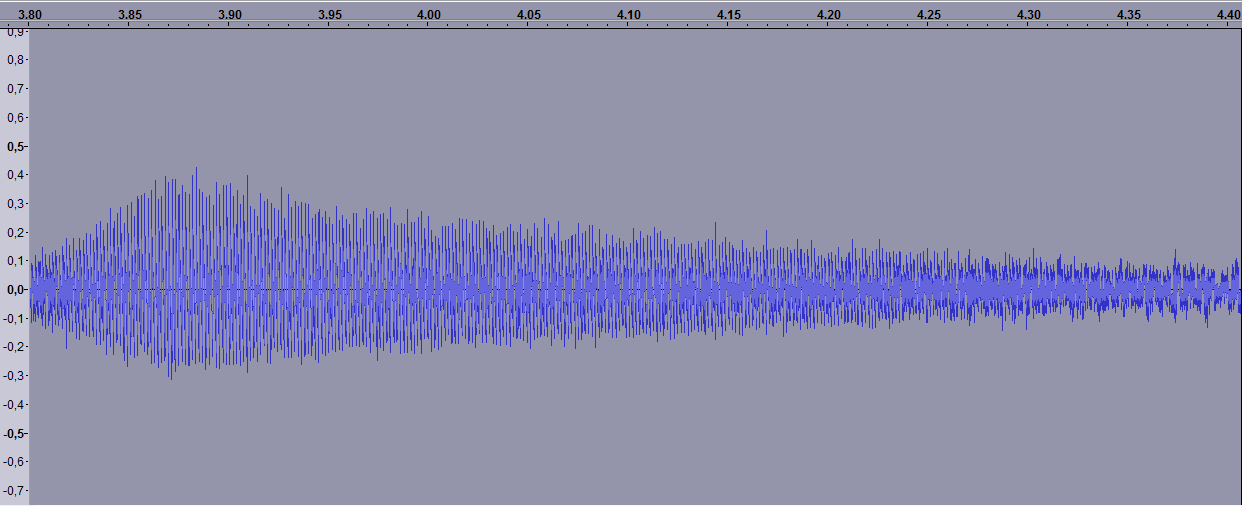
\includegraphics[width = \textwidth]{images/SW5.png}
	\caption{}
	\label{img-sw5}
\end{figure}

\subsubsection{Teleport}
`Teleport' is a SQUARE-based sound effect with the following ADSR envelope:
\begin{itemize}
	\item{Attack: 500 ms}
	\item{Decay: 1250 ms}
	\item{Sustain: 20\%}
	\item{Release: 250 ms}
\end{itemize}
The effect is held for 0 ms.
The total length of the effect is $500 ms + 1250 ms + 250 ms + 0 ms = 2000 ms$.
`Teleport' can be triggered by pressing \texttt{SW4}.
A picture of the recorded sound can be seen in figure \ref{img-sw4}.

\begin{figure}[H]
	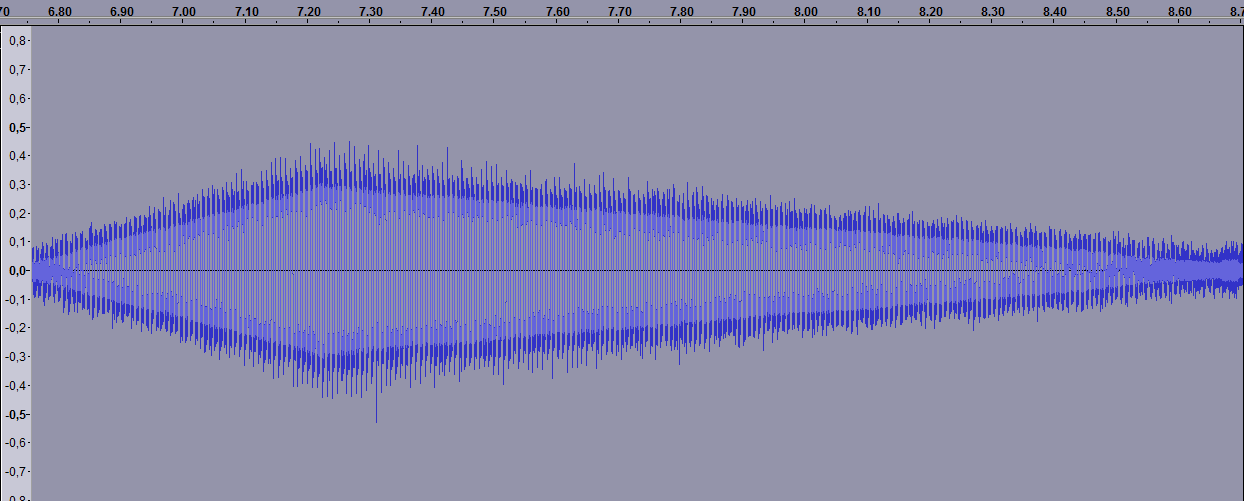
\includegraphics[width = \textwidth]{images/SW4.png}
	\caption{}
	\label{img-sw4}
\end{figure}


\subsection{Music}

The music pieces in the solution program are played by the MOD player.

\subsubsection{Tuulenvire by Dizzy/CNCD}
\emph{Tuulenvire} is a 2:09 long 808KB composition in the ambient genre, featuring piano and accordion, amongst other instruments.
This composition was chosen to demonstrate how careful composing can render realistic compositions with a relatively small memory footprint.
It uses 25 different PCM-coded sounds.
Tuulenvire can be triggered by pressing \texttt{SW3}.

\subsubsection{Boesendorfer P. S. S. by Romeo Knight}
\emph{Boesendorfer P. S. S.} is a 3:22 long 211KB solo piano composition, chosen to illustrate the possibilities enabled by a hybrid generative/recorded approach.
It uses 9 different PCM-coded sounds.
Boesendorfer P. S. S. can be triggered by pressing \texttt{SW2}.

\subsubsection{Drop The Panic by H0ffmann}
\emph{Drop The Panic} is a 4:05 long 702KB ``glitch-hop'' composition.
It was chosen to show how MOD files can support embedded vocals.
It uses 31 different PCM-coded sounds.
The composition was tweaked by adding some extra inaudible notes in the beginning of the song to decrease critical cache misses by the MOD player during playback on the STK1000.
Drop The Panic can be triggered by pressing \texttt{SW1}.

\subsubsection{Bacongrytor by Maktone}
\emph{Bacongrytor} is a 15Kb endless loop chiptune-style composition, chosen to demonstrate the compactness of the MOD format, and therefore its aptfulness for use on microcontrollers.
It uses 7 different PCM-coded sounds.
Bacongrytor can be triggered by pressing \texttt{SW0}.




\section{Solution Components}
	This section describes the solutions' various components.

\subsection{Linux}
The assignment required that the Linux 2.6 kernel be compiled for the AVR32 STK1000 development board.
Specifically, Linux 2.6.16.11-avr32-20060626 was used.

\subsection{Linux Device Drivers for the STK1000}
In the game, STK1000's buttons are used to interface with the user.
The board's LEDs are also used to help with the interface's affordance, highlighting which buttons are available.
Both these actions require interfacing with the hardware of the STK1000, which is something that is unwise to do directly in an application-level program's code base, such as the code base of SLDDD.

This is where a device driver comes in handy. Its job is to provide an abstract interface to the hardware.
Loading device drivers is not straight forward, as they usually reside in kernel space.
Luckily, Linux makes it easy to dynamically load and remove drivers at will.

Many linux drivers, including the ones written for this assignment, allows other programs to interface with hardware through file-like devices.
The user may simply \texttt{fopen} a device, and then write and/or read data to it, using the driver as a middleware translator to translate the write and read calls to whatever is appropriate for the specific device.
\subsubsection{Character device drivers}
    Character device drivers are drivers for character-oriented devices.
    Such a driver transfers data directly to and from a user process.
    The driver written for the LEDs and buttons in this assignment are both of this kind.
\subsubsection{Loading drivers}
When kernel object (.ko) file has been compiled, it may be installed into the kernel with \texttt{insmod <driver>.ko}.
Device drivers require a file-like interface to the hardware, which is generated with the command \texttt{mknod \&dev/<device name> c <major number> <minor number>}.
The major number can be found in \texttt{/proc/devices}, and the minor number is \texttt{0} for the drivers written for this assignment.
A nifty one-liner for inserting a kernel module and making a device node for it as described above is shown in listing \ref{listing-insertmodule}.

LISTING linsting-insertmodule: \texttt{mknod /dev/<device name> c \$(grep <driver> /proc/devices | awk '\{print \$1\}') 0}

Later, to remove a driver, it can be removed using \texttt{rmmod <driver>}, whilst also deleting the device file using \texttt{rm /dev/<device name>}.

\subsubsection{LED driver}
A custom driver was written for the STK1000 to facilitate the turning off and on of the LEDs.
On initialization the driver obtains a major number dynamically and requests a region of memory-mapped hardware before enabling the relevant I/O pins by writing \texttt{0xFF} to the PIO Enable Register (\texttt{PER}) and to the Output Enable Register (\texttt{OER}).

Upon exit, the driver turns the LEDs off by writing \texttt{0xFF} to the Clear Output Data Register (\texttt{CODR}) and \texttt{0x00} to the PIO Enable Register (\texttt{PER}) to disable the I/O pins.
It also releases the region it requested during initialization.

The driver interacts with the LEDs by first turning all the LEDs off (by writing \texttt{0xFF} to the \texttt{CODR}) and then enabling the desired LEDs by writing the given value to the Set Output Data Register (\texttt{SODR}).

For a more detailed explanation of the set-up of the LEDs on the STK1000, see \cite{tdt4258-1}.
For a reference C implementation of this, see \cite{tdt4258-2}.

Noteworthy is the fact that the LEDs no longer reside in PIOC, as in previous assignments \cite{tdt4258-1} and \cite{tdt4258-2}.
This is because PIOC is made unavailable by \texttt{SW6} on the STK1002, see \cite{lab-compendium}.
PIOB is therefore used for both buttons and LEDs.
The LEDs use some of the upper pins of PIOB -- see \cite{lab-compendium}.

\subsubsection{Button driver}
A custom driver was written in order to allow the software to read the buttons' state.

The button driver allows the video game to read the state of the buttons, letting them function as a source of input for the players.
Its initialization is similar to the LED driver's, except that it writes \texttt{0xFF} to the Pull-up Enable Register (\texttt{PUER}) rather than the \texttt{OER}.
Its exit function is similarly different.

The driver reads the button's state by returning the value found in the Pin-Data Status Register (\texttt{PDSR}).

The buttons use the bottom 8 PIOB pins.

For a more detailed explanation of the set-up of the buttons on the STK1000, see \cite{tdt4258-1}. Again, a C reference implementation might exists in \cite{4258-2} TODO: does it? Nope.

\subsubsection{Sound driver}
In order to produce sound, we use the provided ALSA\footnote{Advanced Linux Sound Architecture, see http://www.alsa-project.org/} driver.
This let us simply write raw sound data to \texttt{/dev/dsp} to play it, as described in \cite{lab-compendium}.

The installed linux defaults to muted audio settings, and the lab guidelines recommend using \texttt{alsamixer} to manually set the volume and un-mute it each time the board boots.
Because the authors prefer automating such work, a script is provided that programatically sets the correct audio settings using the more low level \texttt{alsactl}.

TODO: this is just a marker to remind us that we need to deliver the fix_sound.sh script.

\subsubsection{Display driver}
The STK1000 has an LCD screen from Samsung.
It has a resolution of \texttt{320}$\times$\texttt{240} and sports \texttt{32} bits per pixel (\texttt{24} bit color depth, the last \texttt{8} bits are unused)\cite{lab-compendium}.
However, only 24 of these are enabled by default\cite{avr32-disp}.

Data is displayed on the screen by writing a bitmap buffer directly to \texttt{/dev/fb0}.

% should we mention something about orientation?

    \subsection{EGE  - Eeds Game Engine}

    A simple state based game engine was developed specifically for this assignment to ease the development of the solution game.
    The game engine features a simple state system which allows separation of different parts of the program.
    Each state can be thought of almost as a separate program, with separate functions for initializing, deinitializing, updating and so on.
    In the solution game separate states are used for the \textit{splash screen}, the \textit{song selection menu}, the actual gameplay part, and the \textit{score screen}.

    The game engine also is responsible for timers, and makes sure that the game always runs at the same speed independent of CPU load.
    This is done by enforcing a separation of the logical update code and rendering code.
    The idea is that while logical updating at a fixed rate is critical to maintaining temporal consistency in a game, rendering is not.
    Should the logical updating falls behind the schedule, rendering is delayed until the logical updating can catch up with real time again.
    Finally, the game only performs a render if the logical code has signalled that the screen needs a refresh since the last time it was redrawn.
    This is done to save time that would be wasted on drawing the same image to the screen two update cycles in a row.

    The game engine also handles input and output through buttons and LEDs, providing convenient interfaces for the programmer to use.
    The buttons are regularly polled and their state is stored in a global array of boolean values.
    This allows the programmer to simply check the array to see if a button is pressed.
    Button presses can even be simulated programatically by writing to the global button array inbetween polling the buttons.

    The LEDs are exposed through a single function \texttt{set_leds}, which allows the programmer to turn the LEDs on and off.


    Finally, the game engine also supports simple audio playback of raw audio data files.

\subsubsection{Sound}
The sound module of the game engine is capable of playing single raw audio files, as well as controlling the soundcard to set parameters such as bitrate and frequency.
The game engine supports playback of one audio file at a time, which can be set by loading and unloading an audio file to a global pointer.
Mixing, compositing, and other advanced features have not been implented.

\subsubsection{Graphics}
The graphics rendering module is entirely based on bitmaps.
In order to generate the graphics to display to the user, various bitmaps are blitted\footnote{\textit{blit} is an acronym for \textit{bit-level block transfer}.} in order to achieve the desired visual components and effects.


\subsection{``Fontenizer'': the Font Engine}
	A font rendering engine (\texttt{game/include/font.h} and \texttt{game/src/font.c}) was developed in order to easily render some given text on the screen.
	It does this by iterating through a given string\footnote{Actually a C string.} and locating each character's corresponding glyph in a given font bitmap.
	The glyphs are blitted one by one from the font bitmap to a destination bitmap one at a time.
    Variable horizontal character spacing is supported on a per-call basis, allowing for sophisticated kerning.
    Fontenizer supports the basic ASCII character set.
        
\subsection{The \texttt{.SM} file format}
The \texttt{.SM}\footnote{http://www.stepmania.com/wiki/The_.SM_file_format} file format was created by the developers of StepMania, possibly to facilitate the creation and sharing of notes for songs.
An \texttt{.SM}-file contains the dance steps for a song, as well as metadata relating to the song itself (the name of the audio file, the name of the artist and such).

The game engine is capable of reading \texttt{.SM}-files and extracting the relevant data.
Implementing this file format was deemed a feasible alternative to creating notes by hand from scratch, as the popularity of StepMania means there are a wide range of publicly accessible StepMania songs available free of charge on the internet.

\subsection{Tools}

Because manual work is boring and automation is awesome, several tools and scripts were developed to make life easier.
\subsubsection{connect.sh}
This is a script which automatically opens an SSH-connection to the STK1000, without prompting for a password. It can detect when the IP-address of the board has changed, and can find the new address automatically using a thrid party server as a connection broker.

\subsubsection{flashnboot.sh}
This is a script which flashes U-Boot to an STK1000, configures it to boot correctly from an SD-card with the supplied linux SD-image, and then boots the board.
Its primary use is to set up a new board for linux development.

\subsubsection{load\_drivers.sh}
This is a script which automatically loads the drivers and makes the device nodes for the LEDs and buttons on the STK1000.

\subsubsection{fix\_sound.sh}
This is a script which automatically unmutes the STK1000.

\subsubsection{The call-home-script}
This is a script which pings a third party connection broker web server at boot time to let the world know at which IP-address it can be reached.

\subsubsection{Makefiles}
The Makefiles for the drivers and for the game were set up to automatically cross-compile and upload the code from the lab-PCs to the STK1000, and optionally run them as well, without prompting for any user input such as passwords or similar things.



\section{Configuration}
	We can reference our previous report here, so that we don't have to write so much.

\subsection{Jumpers}

As before.

\subsection{GPIO connections}

As before, + maybe mention audio.

\subsection{Audio}

Jack etc
\section{Development of the program}
% Experimental Procedure


\subsection{Sound effect synth}

\subsection{Libmodam}

Libmodam was initially developed in a linux environment on an x86 PC, and later ported to avr32 and the STK1000.
This was done for comfort reasons: there was no need to be in the lab to develop; testing and iterating went a lot faster when code and data didn't need to be uploaded after each modification; and there was no need to focus on performance until features were confirmed to be working properly.
As an added bonus, this also ensured a certain degree of portability, which is a nice property for a library to have.
The python file conversion tool was developed alongside libmodam.

When the code was run on the STK1000 for the first time, the performance difference between the Intel i7 multi-GHz linux laptop and the STK1000 became immediately apparent.
The sound produced by libmodam on the STK1000 at this point did not even remotely sound like music.
In fact, it was more akin to a bowl of half-eaten oatmeal porridge left overnight, were porridge as audibly dull as it is bland in taste.
One of the main reasons for the abysmal performance on the STK1000 was the lack of a floating point unit in the AP7000.
Libmodam used floating point numbers heavily.
The library was rewritten to use integer arithmetic, which helped immensely.
Further optimizations were iteratively applied after this, until the code reached a point of acceptable performance.

\subsection{The main program}

How everything was assembled in the main program.

\subsubsection{Setting up the LEDs}
\subsubsection{Setting up the buttons}
\subsubsection{Setting up the audio}
rant about sample rates, div, diven


list of what we did:

* Board was set up w/ jumpers and such
* Leds and buttons were hooked up in hardware
* Leds and buttons were hooked up in software
* Code was split into separate files
* Audio was hooked up with apropriate settings
* Sound was tested to work using random noise


the following two groups of bullet points happened in parallel:

* a C sound effect synth inspired by sfxr was prototyped on a PC
* the synth was ported to avr32
* the synth was developed further on the avr32
* the synth was used in the stk1000 program to play various sound effects

* a C MOD player library + python tools inspired by amiga trackers were developed on a PC
* the library was tested on the avr32 and needed a great deal of optimization
* a great deal of optimization occurred 
* the library was used in the stk1000 program to play selected mods


finally:

* the actual main program flow was decided upon and written, hooking button and led behaviour together with sound effects and music


\section{Programming Environment}
	
\subsection{JTAGICE}
We can reference our previous report here, so that we don't have to write so much.

\subsection{GNU Debugger}
since last time:
* discovered tui mode: looks nice, breaks the makefile
* avr32gdbproxy -f0.8Mb -a 0.0.0.0:1024 and target extended-remote:1024

\subsection{Make}
we can reference.

\subsection{Other tools}

\begin{itemize}
\item OpenMPT, a MOD tracker, was used to examine MOD files during the development of libmodam.
\item \texttt{vim} was employed as the authors' text editor of choice.
\item \texttt{git} was used for version control.
\item The project was hosted in a private GitHub repository.
\item The report was written with \LaTeX.
\item AVR32-specific flavors of GNU's \texttt{as} and \texttt{ld} were used to assemble and link executables.
\item \texttt{avr32program} was used to program the STK1000 with the JTAGICE.
\item The sound effects were recorded using Audacity on an ASUS UL30JT laptop.
\end{itemize}

table XXX:



For more details about what these effects do, refer to XXX.